\chapter[Referencial teórico]{Referencial Teórico}

Este capítulo apresenta o referencial teórico, que fornece a base para o desenvolvimento deste trabalho. Abordamos os conceitos de prototipação e Design de Serviços (DS), com foco na etapa da prototipação no ciclo de vida do serviço. O segundo tópico de discussão são as principais técnicas e ferramentas de prototipação disponíveis no mercado. Além disso, é abordado o papel do cliente na prototipagem de serviços, visando entender a importância da participação do mesmo na elaboração do protótipo. Por último, é apresentada uma visão geral da prototipação no DS, contextualizando sua relação com outras etapas do processo e destacando sua posição dentro do fluxo geral.

\section{Prototipação}

A prototipação é um processo fundamental no desenvolvimento de novas soluções, produtos ou sistemas. Nesse contexto, modelos preliminares ou representações de ideias são criados para testar conceitos e hipóteses. De maneira geral, a definição de ``protótipo'' é descrita como ``a primeira forma'' \cite{Blomkvist2011existing}, refletindo sua função inicial de representar uma versão inicial de uma ideia para validação e aprimoramento.

Os protótipos manifestam conceitos, ideias ou palpites sobre quais boas soluções podem ser fundadas. Esta é uma maneira de mostrar o conceito e garantir que todos os envolvidos tenham a chance de entendê-lo \cite{Blomkvist2014}.

Portanto, a principal função de um protótipo é testar ideias de maneira prática e concreta, contribuindo para o refinamento e validação de conceitos antes de um investimento significativo na solução ou produto final, cujo custo, na maioria das vezes, é consideravelmente mais alto. Outro ponto não menos importante é que, ao criar protótipos, existe a possibilidade de obter feedbacks valiosos de clientes, usuários e as partes interessadas, trazendo uma segurança a mais de que o produto ou solução desenvolvida esteja alinhado com as expectativas e necessidades.

\subsection{Objetivos}

Seguindo as discussões expostas anteriormente, é possível traçar alguns objetivos principais da prototipação, sendo eles:

\begin{itemize}
	\item \textbf{Visualização de conceitos:} Fazer com que uma ideia ou conceito tenha seu entendimento facilitado entre membros da equipe e partes interessadas.
	
	\item \textbf{Experimentação:} Permitir a experimentação com diversos tipos de soluções e abordagens, fazendo com que problemas e limitações sejam identificados no início.
	
	\item \textbf{Obtenção de feedback:} Coletar opiniões, sugestões e críticas dos usuários e \textit{stakeholders} para ajudar a melhorar e ajustar as soluções em andamento.
\end{itemize}

Esses objetivos mostram como a prototipação tem um papel fundamental no desenvolvimento de soluções eficazes e de acordo com as necessidades do usuário, por exemplo. A visualização de conceitos traz um entendimento mútuo entre todos os envolvidos no projeto, resultando na redução de compreensões distintas ao longo do processo. Já a experimentação traz maiores garantias para que, no momento da implementação final, o processo seja mais tranquilo. Além disso, a obtenção de feedbacks, ao fazer com que os usuários e \textit{stakeholders} atuem ativamente, torna o produto ou serviço mais relevante e funcional.

\subsection{Benefícios}

A prototipação no design de serviços oferece benefícios significativos, como a visualização clara de conceitos, facilitando o entendimento entre a equipe e as partes interessadas. Além disso, permite a experimentação com diferentes soluções, identificando problemas desde as fases iniciais do projeto. Outro benefício importante é a obtenção de feedback valioso de usuários e \textit{stakeholders}, que contribui para o refinamento contínuo da solução, garantindo que ela atenda melhor às necessidades do público-alvo e seja mais eficaz no mercado.



\section{Introdução ao Design de Serviços}

\subsection{Definição}

A definição de DS pode ser algo muito subjetiva, uma vez que muitos autores definem de maneira diferente, além de ser uma área holística, abrangendo muitos processos, atividades e mentalidades. Porém, ainda assim é possível traçar um paralelo entre as definições mais aceitas.

O DS permite que as organizações vejam seus serviços sob a perspectiva do cliente, sendo uma abordagem que busca equilibrar as necessidades dos clientes e do negócio. Seu objetivo é criar experiências de serviço fluidas e de alta qualidade. Fundamentado no \textit{design thinking}, o DS oferece um processo criativo e centrado no ser humano, voltado para a melhoria e o desenvolvimento de novos serviços. Por meio de métodos colaborativos que envolvem tanto clientes quanto equipes de serviço, ele possibilita que as organizações obtenham uma compreensão profunda e abrangente de seus serviços, promovendo melhorias significativas e holísticas \cite{Stickdorn2019}.

Neste sentido, entre os profissionais do Design de Serviços(DS), ainda existem muitas discordâncias em relação às diferenças entre áreas próximas. Assim, existem os defensores de que deve-se separar Design de Serviços(DS) de design de experiência, \textit{design thinking}, experiência do usuário holística, entre outros. Mas também existem aqueles que acreditam que são áreas muito semelhantes, portanto, creem que nomenclaturas não devem ser levadas tão a sério.

\subsection{O que Design de Serviços não é}

Por ser uma área ampla, é importante delimitar o escopo sobre o que não está englobado no DS, para evitar desentendimentos nesse sentido. Logo abaixo são citados alguns tópicos que não são cobertos pelo DS:

\begin{itemize}
	\item \textbf{Não é estética}: Designers de serviços se preocupam muito mais com o funcionamento e a criação de valor do que com a boa aparência do serviço.
	
	\item \textbf{Não é ``atendimento ao cliente''}: É justamente o que ele visa evitar, uma vez que, quanto melhor e mais intuitivo o serviço, menos suporte o cliente precisará, logo diminuindo a questão do atendimento ao cliente.
	
	\item \textbf{Não é ``recuperação de serviço''}: Muito pelo contrário, o DS deve ser utilizado durante o processo de criação, e não quando o produto/serviço já deu errado e precisa de alguma salvação milagrosa.
\end{itemize}

\subsection{Princípios do Design de Serviços}

Existe uma discussão sobre o que são os princípios de fato do Design de Serviços (DS). Isso ocorre devido a diversos fatores, mas o principal deles foi a reunião de cinco princípios fundamentais no livro ``Isto é design de serviço'', lançado em 2010. Esses princípios foram fortemente difundidos, porém se fez necessário uma revisão dos mesmos, uma vez que alguns ficaram um pouco defasados com o tempo. Nesse ponto, acaba havendo um descompasso entre os princípios presentes nesse livro e os princípios mais condizentes com a realidade. Esses eram os princípios:

\begin{itemize}
	\item \textbf{Centrado no usuário}: serviços devem ser testados através do olhar do cliente.
	\item \textbf{Cocriativo}: todos os \textit{stakeholders} devem ser incluídos no processo do desenho do serviço.
	\item \textbf{Sequenciado}: o serviço deve ser visualizado como uma sequência de ações inter-relacionadas.
	\item \textbf{Evidente}: serviços intangíveis devem ser visualizados por meio de suas evidências físicas.
	\item \textbf{Holístico}: todo o ambiente de um serviço deve ser levado em consideração.
\end{itemize}

Alguns dos princípios necessitaram de uma breve modificação, sendo de uma palavra ou outra, já outros, tiveram que passar por uma reformulação mais significativa.

O primeiro, ao ser nomeado como \textbf{``centrado no usuário''} traz uma interpretação de que pode-se excluir alguns grupos que também interagiam com o sistema, como a equipe interna, por exemplo. Logo, no lugar de \textbf{``usuário''}, fez mais sentido a utilização de \textbf{``ser humano''} para assim englobar de forma mais adequada todos os grupos.

O segundo, ao ser chamado de \textbf{``Cocriativo''}, é o resultado da união de dois conceitos, \textbf{``cocriação''} e \textbf{``\textit{codesign}''}. O primeiro trabalha no sentido de valor gerado por serviços, já o segundo traz uma ideia do ``processo de criação feito por um grupo de pessoas, normalmente vindas de diferentes contextos'' \cite{Stickdorn2019}. Porém, com o tempo, o foco foi mais direcionado para esse segundo conceito.

O terceiro, com a nomenclatura de \textbf{``Sequenciado''}, faz referência à importância da relação entre os vários momentos de contato com o serviço. Neste caso, a mudança necessária foi somente para o melhor entendimento do princípio, não mudando nada no seu significado original, uma vez que a palavra ``sequenciado'' não é comum no cotidiano das pessoas.

O quarto, titulado de \textbf{``Evidente''}, reconhece a intangibilidade de algumas partes do serviço, destacando sempre o valor do serviço em si, mesmo que não exista uma maneira clara e tangível de avaliar essa importância.

O quinto, conceituado de \textbf{``Holístico''}, foi chamado assim por basicamente reunir muitos conceitos em uma palavra só. Ao defender essa reunião de conceitos como ``a relevância de todos os nossos sentidos para uma experiência de serviço; outro é a ampla variedade de jornadas individuais que um serviço pode gerar; e o último trata da relevância do Design de Serviços para a identidade corporativa e para as metas de uma organização'' \cite{Stickdorn2019}.

Outro ponto importante é que, nesses cinco princípios originais, não houve ênfase em uma característica fundamental do Design de Serviços, a \textbf{iteração}. A iteração se diz respeito a começar com tentativas que não visam a perfeição, mas sim a simplicidade, e com base nisso, naturalmente haverão falhas. Com essas falhas, lições devem ser aprendidas para que as próximas tentativas sejam melhores, ou seja, aprender com as falhas.

Com base nesses pontos de revisão e melhoria, os seguintes novos princípios de Design de Serviços surgiram \cite{Stickdorn2019}:

\begin{itemize}
	\item \textbf{Centrado no ser humano}: considera a experiência de todas as pessoas afetadas pelo serviço.
	\item \textbf{Colaborativo}: \textit{stakeholders} advindos de contextos e funções variados devem se envolver ativamente no processo de desenho de um serviço.
	\item \textbf{Iterativo}: o DS é uma abordagem exploratória, adaptativa e experimental, que promove a iteração do protótipo de um serviço rumo à sua implementação.
	\item \textbf{Sequencial}: o serviço deve ser visualizado e regido como uma sequência de ações inter-relacionadas.
	\item \textbf{Real}: as necessidades do usuário devem ser pesquisadas no mundo real, as ideias devem ser prototipadas no mundo real e os valores intangíveis devem ser postos em evidência por meio de uma realidade física ou digital.
	\item \textbf{Holístico}: devem ser consideradas, de modo sustentável, as necessidades de todos os \textit{stakeholders} ao longo do serviço e a interação com todas as facetas do negócio.
\end{itemize}

Resumidamente, o Design de Serviços ``é uma abordagem centrada no ser humano, colaborativa, interdisciplinar, iterativa, que utiliza pesquisa, prototipação e um conjunto de atividades e ferramentas de visualização de fácil entendimento para criar e orquestrar experiências que atendam às necessidades do negócio, do usuário e dos \textit{stakeholders} do serviço'' \cite{Stickdorn2019}.

\begin{figure}[h]
	\centering % para centralizarmos a figura
	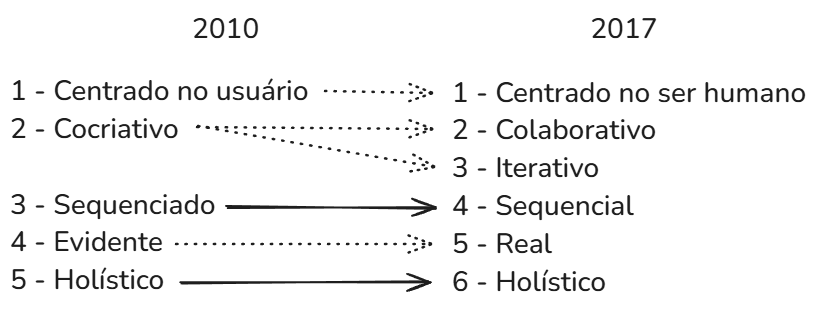
\includegraphics[width=16cm]{figuras/principios.png} % leia abaixo
	\caption{Transição dos princípios do design de serviço}
	Fonte: Elaboração própria
	\label{figura:qualquernome}
\end{figure}

\subsection{Lógica serviço-dominante}

Uma organização, independentemente do setor econômico em que opera, sempre terá seu produto fundamental como serviço. Independentemente do produto, sempre será um serviço, pois todos os produtos têm sua criação baseada em processos de Design de Serviços \cite{Stickdorn2019}.

Nesse sentido, é importante compreender a lógica serviço-dominante (S-D), pois ela demonstra de fato que os serviços são o início, meio e fim de qualquer atividade econômica. Essa lógica é pautada em 11 premissas, que são divididas em 5 axiomas primordiais, sendo eles:

\begin{enumerate}
	\item O serviço é a base fundamental de transação.
	\item O valor é cocriado por múltiplos atores, incluindo o beneficiário.
	\item Todos os atores sociais e econômicos são integradores de recursos.
	\item O valor é sempre único e fenomenologicamente determinado pelo beneficiário.
	\item A cocriação de valor é coordenada por meio de instituições e arranjos institucionais gerados por atores.
\end{enumerate}

Esses axiomas facilitam o entendimento de todos os produtos como serviço, pois oferecem uma base para entender como os bens, sejam físicos ou intangíveis, se transformam quando são oferecidos de forma contínua e sob demanda. Com esses princípios, fica mais fácil perceber como as empresas ajustam seus modelos de negócios para focar na experiência do cliente, em vez de simplesmente entregar um produto pronto. Esse modelo não só torna os produtos mais flexíveis, como também cria uma relação mais dinâmica entre fornecedor e cliente, com ênfase no serviço contínuo e personalizado.

Entre esses axiomas, o 5º ganha um destaque importante, pois a partir dele, é possível construir uma definição direta do significado de Design de Serviços. Pode-se dizer que Design de Serviços é o processo de coordenar instituições e arranjos institucionais para possibilitar a cocriação de valor.

Com os pontos apresentados, é notável a importância da lógica S-D para o Design de Serviços. Conforme a lógica S-D se desenvolve, ela traz cada vez mais à tona características importantes do serviço em si, além do entendimento de qualquer produto como um serviço.

\subsection{Os 12 mandamentos do \textit{design de serviços}}

De acordo com \citeonline{Stickdorn2019}, os ``12 Mandamentos da Prática do Design de Serviços'' oferecem diretrizes práticas e centradas no usuário. Eles podem ser descritos como:

\begin{enumerate}
	\item \textbf{Chame-o como preferir}
	
	Existem muitas nomenclaturas para o DS, porém não se deve se preocupar com a forma como será chamado, o importante é aplicar os conceitos.
	
	\item \textbf{Faça os primeiros rascunhos grosseiros}
	
	As primeiras versões de um serviço não devem se preocupar com beleza nem com muito detalhamento.
	
	\item \textbf{Você é um facilitador}
	
	A principal preocupação de um designer de serviços é manter a equipe e os clientes trabalhando juntos.
	
	\item \textbf{Não diga, faça}
	
	Como o DS é baseado na realidade, construir e testar é mais importante do que perder muito tempo falando sobre algo, por exemplo.
	
	\item \textbf{``Sim, mas...'' e ``Sim, e...''}
	
	São duas técnicas interessantes: uma para o início do desenvolvimento, onde se busca expandir as opções e ideias, e a outra para o desenvolvimento posterior, onde se busca limitar as ideias para desenvolvê-las.
	
	\item \textbf{Encontre o problema certo antes de resolvê-lo da forma certa}
	
	É mais importante ter o problema claramente definido do que sair procurando soluções para um problema que talvez nem seja o correto.
	
	\item \textbf{\textit{Prototipe} no mundo real}
	
	É muito importante testar as ideias no mundo real, construindo e testando principalmente. Isso porque as ideias quando estão na mente podem parecer perfeitas, mas na prática, pode não serem tão boas assim.
	
	\item \textbf{Não coloque todos os ovos na mesma cesta}
	
	Sempre utilize diversos métodos e pontos de vista para as pesquisas, além de apostar em vários protótipos.
	
	\item \textbf{Não se trata de usar ferramentas, mas de mudar a realidade}
	
	Um projeto de DS vai além da ideação e documentação inicial, exigindo execução, iteração e entendimento profundo das necessidades reais dos envolvidos.
	
	\item \textbf{Planeje para a iteração; depois, adapte}
	
	O planejamento é fundamental, porém o mesmo não deve ser engessado, deve permitir adaptações conforme necessário.
	
	\item \textbf{Amplie e minimize}
	
	O DS ultrapassa a etapa de ideação e documentação, demandando ações práticas, revisões contínuas e uma compreensão verdadeira das necessidades dos envolvidos.
	
	\item \textbf{Tudo é serviço}
	
	Os conceitos e práticas do DS podem ser aplicados a tudo, não se trata apenas de deixar os clientes felizes.
	
\end{enumerate}

\section{Prototipação no Design de Serviço}

A prototipação, como abordada anteriormente, é um processo essencial para o desenvolvimento de soluções eficazes e alinhadas às necessidades dos usuários e \textit{stakeholders}.No contexto do Design de Serviços (DS), a prototipação desempenha um papel crucial, pois permite que conceitos intangíveis sejam representados de forma concreta, facilitando o entendimento e a comunicação entre as partes envolvidas. De acordo com \citeonline{Stickdorn2019}, a prototipação no DS é essencial para testar hipóteses, visualizar experiências e iterar soluções com base no feedback dos usuários. Essa relação é fundamentada na natureza iterativa tanto da prototipação quanto do DS, permitindo ajustes contínuos para garantir que o serviço final atenda às expectativas dos clientes e às necessidades do negócio.

%No \textit{design de serviço}, os protótipos não são apenas representativos do resultado final; eles também atuam como ferramentas exploratórias que ajudam a identificar pontos de melhoria ao longo do ciclo de vida do serviço. A prototipação iterativa é essencial neste processo, pois permite que cada versão do protótipo seja refinada com base no feedback coletado. Como descrito por Christie em \textit{Prototyping Strategies: Literature Review and Identification of Critical Variables}, "a iteração é a sequência de testes e aprimoramentos sucessivos de um protótipo, permitindo que ele evolua gradualmente até atender aos requisitos esperados"\cite{Christie2012}.

Além disso, a prototipação no DS contribui para a cocriação, um dos princípios centrais da área. Envolver \textit{stakeholders} no desenvolvimento dos protótipos permite que suas perspectivas sejam incorporadas ao \textit{design}, promovendo soluções mais holísticas e centradas no ser humano. Essa abordagem colaborativa é particularmente relevante quando se trata de serviços, que frequentemente envolvem uma ampla gama de interações e experiências, tanto físicas quanto digitais.

Outro aspecto significativo é a capacidade de evidenciar e sequenciar experiências do serviço por meio da prototipação. Protótipos permitem visualizar e organizar as várias etapas e pontos de contato do serviço, garantindo que cada um seja projetado de maneira integrada e eficiente. Isso é particularmente útil para alinhar as equipes internas e gerar \textit{insights} práticos sobre como os clientes interagem com o serviço em diferentes contextos.

Ou seja, o DS utiliza a prototipação como um meio de tornar tangíveis aspectos intangíveis, como fluxos de experiência, jornadas do cliente e processos internos. Ao testar essas ideias no mundo real, o DS não apenas mitiga riscos, mas também maximiza as chances de criar soluções que atendam às necessidades dos usuários de forma eficaz e inovadora. Essa abordagem iterativa e centrada no ser humano demonstra como a prototipação não é apenas uma ferramenta, mas uma parte integral do processo criativo no DS.

Em suma, no DS, a prototipação é uma forma de testar, explorar e visualizar como as pessoas podem vivenciar ou interagir com um serviço ou situação no futuro. Segundo \cite{Stickdorn2019}, os protótipos desempenham um papel essencial ao ajudar a equipe de \textit{design} a compreender e refinar soluções. A seguir, serão abordados mais detalhes sobre como a prototipação contribui para o processo de \textit{design} e os diferentes tipos de protótipos que podem ser utilizados.

\begin{itemize}
	\item Identificar rapidamente aspectos importantes de um novo conceito de serviço e explorar diferentes alternativas de solução.
	\item Avaliar sistematicamente quais soluções podem funcionar na realidade diária.
	\item Criar um entendimento compartilhado de conceitos e ideias iniciais, melhorando a comunicação, colaboração e participação de \textit{stakeholders} interdisciplinares.
\end{itemize}

A prototipação desempenha um papel fundamental na redução ágil de riscos e incertezas durante o desenvolvimento de um projeto. Nesse contexto, ela se destaca como a abordagem mais econômica e eficiente para identificar e solucionar os problemas identificados.

Além disso, a prototipação não se limita apenas à resolução de problemas; ela também pode ser utilizada como a etapa inicial de um projeto. Nesse estágio, sua aplicação frequentemente gera diversas ideias e questionamentos, o que contribui significativamente para o processo de pesquisa e ideação da equipe.

Durante o desenvolvimento de um projeto de DS, diferentes métodos de prototipação são aplicados de acordo com a fase do projeto. No início, por exemplo, costuma-se utilizar métodos mais simples, como a prototipação de baixa fidelidade, que permitem explorar conceitos de forma rápida e econômica. Já nas etapas finais, simulações e testes com protótipos de alta fidelidade, mais próximos da realidade, tornam-se mais adequados para validar as soluções propostas.

De acordo com \cite{Christie2012}, a prototipação no DS é essencialmente um processo iterativo. Em vez de buscar a criação de um único protótipo final, a abordagem iterativa visa o desenvolvimento de várias versões de um protótipo, refinando-o continuamente com base nos testes e no feedback coletado. Esse ciclo de testes e aprimoramentos permite que o protótipo evolua gradualmente, até atender plenamente aos requisitos esperados.

\subsection{Atividades}

É válido ressaltar que as atividades listadas a seguir não precisam, necessariamente, ser seguidas de forma rigorosa. Elas servem apenas como uma orientação flexível, permitindo adaptações conforme as necessidades e características específicas de cada projeto.

\subsubsection{Decisão do propósito}

Naturalmente, a primeira atividade é definir a finalidade do protótipo. Além do motivo de sua criação, é importante também definir o que se deve alcançar com a criação do mesmo.

Segundo \cite{Stickdorn2019}, as três principais razões pelas quais a prototipação é usada no Design de Serviço (DS) são explorar, avaliar e se comunicar. É válido ressaltar que essas razões podem se misturar, mesmo em uma única sessão de prototipação.

\begin{itemize}
	\item \textbf{Explorar}
	
	É basicamente quando o objetivo da prototipação é criar novas soluções ou obter novas ideias a partir de um conceito inicial. Pode ser usado como uma forma de ideação. Neste momento os protótipos são feitos para serem descartáveis, então é interessante utilizar materiais e plataformas voltadas para criação rápida de protótipos.
	
	\item \textbf{Avaliar}
	
	Ao contrário da prototipação exploratória, aqui o objetivo principal é convergir as ideias. Ou seja, o foco é em reduzir o número de opções disponíveis, visando refinar o foco do projeto. Neste momento os protótipos são construídos para serem apresentados a clientes e \textit{stakeholders}, então o foco é na criação de um protótipo mais fiel possível ao serviço.
	
	\item \textbf{Se comunicar}
	
	Aqui, o objetivo é criar um protótipo para apresentar para um público mais amplo. A ideia é tirar possíveis dúvidas sobre o serviço com a demonstração por meio do protótipo. Pode ser usado até para auxiliar em apresentações sobre o serviço.
\end{itemize}

\subsubsection{Decisão sobre quais são as perguntas de prototipação}

A elaboração das perguntas é uma atividade muito importante pois ela deixa claro e objetivo o que se quer aprender ou realizar com a atividade. As perguntas devem servir como um guia para a etapa da prototipação.

Segundo \cite{Stickdorn2019}, existem quatro perspectivas importantes para gerar essas perguntas iniciais: o \textbf{valor}, a \textbf{aparência}, a \textbf{viabilidade} e a \textbf{integração}. 

Ao levar essas perspectivas em consideração ao formular as perguntas, a chance da equipe ter os mesmos objetivos com a prototipação aumenta consideravelmente.

\subsubsection{Avaliação do que fazer ou construir}

Como cada protótipo não precisa necessariamente ter o serviço representado em sua totalidade, é importante que seja definido quais partes do serviço/produto estarão sendo representadas no protótipo em questão. A utilização de um portfólio de protótipos pode ser uma estratégia interessante nesse aspecto, visando discutir sobre quais elementos do serviço vão ser representados naquele protótipo em questão.

\subsubsection{Planejamento da prototipação}

O planejamento das atividades de prototipação é uma etapa muito dependente de quais são as perguntas de prototipação. Isso acontece pois aqui, o planejamento das atividades a serem realizadas deve ser feito da maneira mais proveitosa possível para as perguntas.

Muitos aspectos são relevantes no momento do planejamento da prototipação, segundo \cite{Stickdorn2019}, são eles:

\begin{itemize}
	\item \textbf{Público}
	
	Basicamente a amostragem daquele protótipo, definir quem usará, quem será observado, quem deve participar das sessões de prototipação.
	
	\item \textbf{Autores}
	
	Aqui são definidos os papéis da equipe que conduz a atividade da prototipação, cada indivíduo pode possuir mais de um papel

\item \textbf{Fidelidade}

Neste momento, é definido o nível de detalhamento que o protótipo terá. Isso está ligado de forma direta com as questões econômicas, uma vez que, quanto mais detalhado o protótipo for, mais tempo demora para ser feito e, como consequência, mais dinheiro é gasto.

\item \textbf{Contexto}

O contexto faz referência direta ao ambiente onde as sessões de prototipação serão executadas. Segundo \cite{Stickdorn2019}, existem duas abordagens principais: a prototipação contextual e a prototipação em laboratório.

A prototipação contextual é feita no local onde o serviço seria usado, ou seja, um ambiente sem muito controle. Já a prototipação em laboratório é feita em um ambiente mais controlado, utilizada quando não é possível testar no contexto real do serviço. Um quesito importante é que, quanto mais próximo do contexto real, mais confiáveis e valiosos são os feedbacks obtidos a partir daquela sessão.

\item \textbf{Rodadas de prototipação}

Este tópico tem muita relação com a questão da iteração. O planejamento da prototipação precisa ser feito pensando em rodadas de prototipação, ou seja, uma sequência de ciclos ou rodadas de prototipação.

Isso pode gerar uma complexidade maior no planejamento, pois cada ciclo deve ter um objetivo bem definido para que, a partir dele, sejam gerados \textit{insights} mais objetivos. Geralmente, as primeiras rodadas são mais exploratórias, e depois o refinamento passa a se tornar o objetivo.

\item \textbf{Monitoramento múltiplo}

No processo de prototipação, é necessário decidir quantos protótipos desenvolver em cada área. Dividir as tarefas em várias frentes ajuda a reduzir riscos e evita concentrar tudo em um único projeto. Isso também facilita o gerenciamento da incerteza do portfólio de ideias e das expectativas dos envolvidos.

Além disso, é importante decidir se equipes diferentes trabalharão em protótipos distintos ou se uma única equipe ficará responsável por todos, um de cada vez. A fase de prototipação inclui várias etapas, com sessões de testes e ajustes que podem ocorrer simultaneamente ou em sequência.

\item \textbf{Seleção de método}

Por último, vem a seleção do método. Essa seleção depende de muitos fatores citados anteriormente, como fidelidade e contexto, por exemplo. De maneira mais geral, segundo \cite{Stickdorn2019}, é válida a inclusão de pelo menos um método de cada uma das seguintes categorias: Validação da proposta de valor original, exploração e avaliação segundo uma perspectiva holística e elementos-chave.	
	
\end{itemize}

\subsubsection{Sessões de prototipação}

Existem diversos métodos de prototipação, porém todos eles possuem uma estrutura muito semelhante, segundo \cite{Stickdorn2019} eles podem ser divididos em três atividades principais, sendo elas:

\begin{itemize}
	\item \textbf{Preparação}: Primeira atividade, nela deve-se preparar os protótipos por meio da maneira mais adequada, seja ela por modelos ou canvas, criação de modelos físicos, etc.
	
	\item \textbf{Aplicação}: Segunda atividade, onde se utiliza o que foi preparado na primeira fase para explorar, avaliar ou comunicar o conceito de design objetivado.
	
	\item \textbf{Pesquisa}: Terceira e última fase, onde se obtém os feedbacks e \textit{insights} gerados pelo protótipo.
\end{itemize}

É importante ressaltar que prototipar não é somente a atividade de criação do protótipo, essa é apenas a primeira atividade. Talvez a parte mais valiosa da prototipação são os \textit{insights} e feedbacks obtidos a partir do protótipo em si.

\subsubsection{Síntese e análise de dados}

Após a execução das sessões de prototipação, muitos dados e \textit{insights} são gerados. Essa etapa é responsável por tratar e sintetizar esses dados para que os mesmos sejam úteis de alguma maneira para o projeto.

\subsubsection{Visualização de dados de prototipação}

Por fim, a visualização dos dados é a maneira com que os dados obtidos serão apresentados, para isso existem diversas técnicas como mural de pesquisa, personas, mapas de jornada, mapas de \textit{stakeholders}, \textit{insights}-chave dentre outros.

%\section{Técnicas e ferramentas} -> Vai ser resultado

%\section{Papel do cliente} -> Vai ser resultado

%\section{Contexto}
